\section{Experiments}

We use 90\% of our labeled documents as train and test on the remaining 10\%. Since revision history data is noisy, we manually go through our test data to discard documents that have incorrect infobox  labels by looking the  text that  changed. The task is to predict for each document (revision), the label (infobox slot change) of the document given its verbs features. We compute precision, recall, and F1 values of our predictions  and compare the values before and after feature selection (Fig. \ref{fig:result}).

%\begin{table}
%\begin{small}
%\begin{center}
%\begin{tabular}{|l|r|r|r|}
%\hline
%Method & Precision & Recall & F1 \\
%\hline
%\textsc{MaxEnt} & 0.82 & 0.79 & 0.80 \\
%\hline
%\textsc{MaxEnt} + MIP & 0.88 & 0.76 & 0.82 \\
%\hline
%\end{tabular}
%\caption{\label{table:performance} Results of predicting state change label using verb features.}
%\end{center}
%\end{small}
%\end{table}

We observe the value of doing feature selection by asserting constraints in an MIP formulation in Figure \ref{fig:result}. Feature selection improves precision; resulting in a better F1. By asserting constraints, some of the  inconsistent verb features for the labels were removed. For example, before feature selection, the verbs: ``marry", and ``be married to" were high-weighted features for both \textit{begin-spouse} and \textit{end-spouse}. After asserting constraints that \textit{begin-spouse} is mutex with \textit{end-spouse}, these verbs (whose base form is ``marry") are filtered out from the features of \textit{end-spouse}. We show some of the learned verb features (after feature selection) for some of the labels in (Table \ref{table:verbs}). In average, we learn about 18 verbs per infobox state change in our state changing verb resource. 

\begin{figure}
\begin{center}
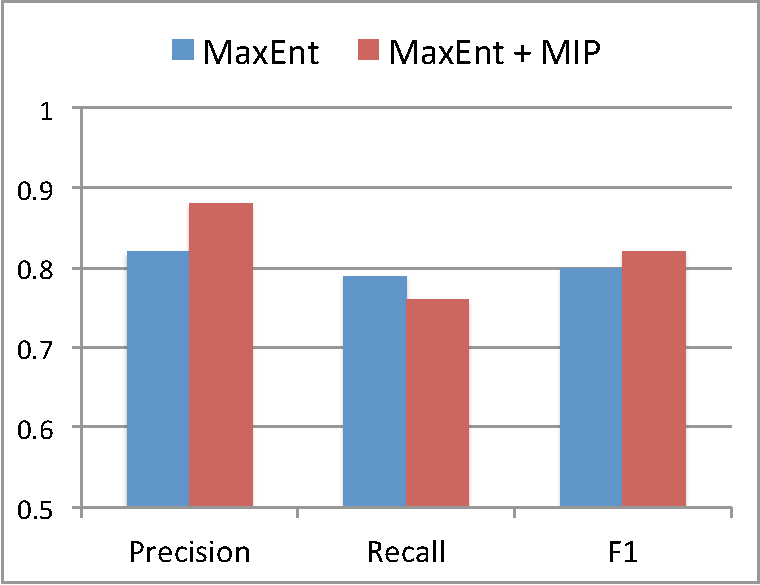
\includegraphics[width=5cm,keepaspectratio=true]{figures/result.pdf}
\caption{\label{fig:result} Results of predicting state change labels (infobox types) using verb features.}
\end{center}
\end{figure}

\begin{table}[t]
\begin{scriptsize}
\begin{center}
\begin{tabular}{|l|l|}
\hline
Label & Verb \\
\hline
\textit{begin-} &+(arg1) die on (arg2), +(arg1) die (arg2), \\
\textit{deathdate}& +(arg1) pass on (arg2) \\
\hline
%\textit{begin-deathplace} &+(arg1) die in (arg2), +(arg1) die at (arg2), +(arg1) move to (arg2) \\
%\hline
\textit{begin-} &+(arg1) be born in (arg2), +(arg1) bear in (arg2), \\
\textit{birthplace}&+(arg1) be born at (arg2) \\
\hline
\textit{begin-} &+(arg1) succeed (arg2), +(arg1) replace (arg2), \\
\textit{predecessor}& +(arg1) join cabinet as (arg2), +(arg1) join as (arg2) \\
\hline
\textit{begin-} &+(arg1) lose \textbf{seat} to (arg2), +(arg1) resign on (arg2), \\
\textit{successor}& +(arg1) resign from post on (arg2) \\ %+(arg1) lose election to (arg2) \\
\hline
%\textit{begin-} &+(arg1) work as (arg2), +(arg1) nominate for (arg2), \\
%\textit{occupation}& +(arg1) establish as (arg2) \\
%\hline
\textit{begin-} &+(arg1) be appointed on (arg2), +(arg1) serve from (arg2), \\
\textit{termstart}& +(arg1) be elected on (arg2) \\
\hline
%\textit{begin-termend} &+(arg1) resign on (arg2), +(arg1) step down in (arg2), \\
%& +(arg1) flee in (arg2) \\
%\hline
%\textit{begin-office} &+(arg1) be appointed as (arg2), \\
%& +(arg1) serve as (arg2), +(arg1) be appointed (arg2) \\
%\hline
\textit{begin-} &+(arg1) marry on (arg2), +(arg1) marry (arg2), \\
\textit{spouse}& +(arg1) be married on (arg2), -(arg1) be engaged to (arg2) \\
\hline
\textit{end-spouse} &+(arg1) file \textbf{for divorce} in (arg2), +(arg1) die on (arg2), \\
& +(arg1) divorce in (arg2) \\%+(arg1) announce \textbf{separation} on (arg2) \\
\hline
%\textit{begin-children} &+(arg1) have \textbf{child} (arg2), +(arg1) raise daughter (arg2), \\
%& +(arg1) raise (arg2) \\
%\hline
%\textit{begin-party} &+(arg1) launch (arg2), +(arg1) be elected as (arg2), +(arg1) be elected (arg2) \\
%\hline
%\textit{begin-} &+(arg1) graduate from (arg2), +(arg1) attend (arg2), \\
%\textit{almamater}& +(arg1) be educated at (arg2) \\
%\hline
%\textit{begin-awards} &+(arg1) be awarded (arg2), +(arg1) be named on (arg2), \\
%& +(arg1) receive (arg2) \\
%\hline
\textit{begin-} &+(arg1) start career with (arg2), \\
\textit{youthclubs}& +(arg1) begin \textbf{career} with (arg2), +(arg1) start with (arg2) \\
\hline
%\textit{begin-clubs} &+(arg1) play for (arg2), +(arg1) play during career with (arg2),\\
%& +(arg1) sign with (arg2), +(arg1) complete \textbf{move} to (arg2) \\
%\hline
%\textit{begin-} &+(arg1) make \textbf{appearance} for (arg2), \\
%\textit{nationalteam}& +(arg1) make debut for (arg2), +(arg1) play for (arg2) \\
%\hline
\end{tabular}
\caption{\label{table:verbs} Comparison of verb phrases learned before and after feature selection for various labels (infobox types).}
% The texts in bold are (prep+) noun that occur most frequently with the combination of the (verb, label) in the train data.}
\end{center}
\end{scriptsize}
\end{table}
\normalsize
